\section{Visualizing Profiler Outputs}

Several useful plotting methods have been provided in the \pkg{pbdPROF} package for visualizing fpmpi and mpiP profiler outputs.  

In addition, the data is stored in a fairly simple format, so it should be simple enough to create your own plots if these do not suffice.

\subsection{Visualizing fpmpi Profiler Output}

An example parsed fpmpi dataset is included in the \pkg{pbdPROF} package, called \code{fpmpi_example}.  It contains the profiler output of the fpmpi library example \code{prof_test}, located in the example subtree of the library source.  The example was run with 4 processors, and the parsed profiler output is as follows:
\begin{Output}
An fpmpi profiler object:
$Routine
[1] "MPI_Allreduce" "MPI_Recv"      "MPI_Send"      "MPI_Barrier"  

$Calls
[1] 1 1 1 2

$Time
[1] 8.46e-06 4.05e-06 1.91e-06 1.75e-05

$Data.Sent
[1] 40 40 40  0

$SyncTime
[1] 3.46e-06 0.00e+00 0.00e+00 0.00e+00
\end{Output}

\begin{figure}[h]
  \centering
  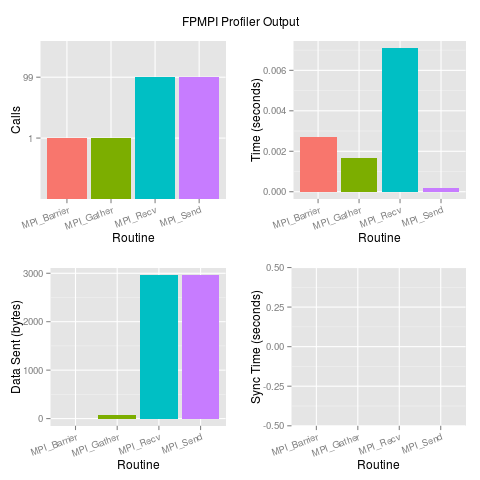
\includegraphics[width=0.7\textwidth]{include/pics/fpmpi}
  \caption{fpmpi Plots}
  \label{fig:fpmpi}
\end{figure}

The package includes some default plots which can easily be produced, either by \code{plot()} or \code{autoplot()} calls.  Figure~\ref{fig:fpmpi} shows the plots which can be produced from the following script.
\begin{lstlisting}[language=rr]
> library(pbdPROF)
> x <- fpmpi_example
> plot(x)
\end{lstlisting}


\subsection{Visualizing mpiP Profiler Output}

An example parsed mpiP dataset is included in the \pkg{pbdPROF} package, called \code{mpip_example}.  It contains the profiler output of the mpiP library example \code{11-p2p-mess-size.exe}, located in the testing subtree of the library source.  The example was run with 4 processors, and the parsed profiler output is as follows:
\begin{Output}
An mpip profiler object:
[[1]]
  Task AppTime MPITime  MPI.
1    0  0.0192 0.00753 39.28
2    1  0.0195 0.00740 37.98
3    2  0.0194 0.00765 39.35
4    3  0.0194 0.00368 18.95
5    *  0.0775 0.02630 33.88

[[2]]
   ID Lev File.Address Line_Parent_Funct      MPI_Call
1   1   0      4225651         [unknown]          Recv
2   2   0      4226678         [unknown]          Recv
3   3   0      4225914         [unknown]          Recv
4   4   0      4226382         [unknown]          Recv
5   5   0      4226540         [unknown]       Barrier
6   6   0      4226080         [unknown]         Irecv
7   7   0      4225924         [unknown]       Barrier
8   8   0      4226816         [unknown]          Recv
9   9   0      4226530         [unknown]         Irecv
10 10   0      4225661         [unknown]       Barrier
11 11   0      4226236         [unknown]          Recv
12 12   0      4226090         [unknown]       Barrier
13 13   0      4225988         [unknown]       Barrier
14 14   0      4225807         [unknown]        Ibsend
15 15   0      4225526         [unknown] Buffer_attach
16 16   0      4225762         [unknown] Buffer_attach
17 17   0      4226631         [unknown]          Send
18 18   0      4226446         [unknown]       Barrier
19 19   0      4226335         [unknown]        Issend
20 20   0      4225836         [unknown]          Wait
21 21   0      4226033         [unknown]        Irsend
22 22   0      4226769         [unknown]         Ssend
23 23   0      4225563         [unknown]         Bsend
24 24   0      4225817         [unknown]       Barrier
25 25   0      4226483         [unknown]         Rsend
26 26   0      4226189         [unknown]         Isend
27 27   0      4225855         [unknown] Buffer_detach
28 28   0      4225592         [unknown] Buffer_detach
29 29   0      4225573         [unknown]       Barrier

[[3]]
            Call Site  Time App.  MPI.  COV
1        Barrier   10 6.930 8.94 26.37 1.41
2        Barrier   24 6.420 8.28 24.45 0.85
3        Barrier    7 5.140 6.63 19.56 1.41
4           Recv    1 2.440 3.15  9.29 0.97
5  Buffer_attach   15 2.250 2.91  8.59 0.99
6        Barrier   29 1.730 2.23  6.57 1.37
7        Barrier   12 0.205 0.26  0.78 0.12
8        Barrier   18 0.191 0.25  0.73 0.01
9           Recv    2 0.128 0.17  0.49 0.29
10          Recv    3 0.114 0.15  0.43 1.14
11          Wait   20 0.090 0.12  0.34 0.00
12         Bsend   23 0.084 0.11  0.32 0.71
13       Barrier    5 0.071 0.09  0.27 1.25
14          Recv   11 0.065 0.08  0.25 0.72
15         Ssend   22 0.062 0.08  0.24 0.64
16 Buffer_detach   28 0.054 0.07  0.21 0.84
17         Rsend   25 0.053 0.07  0.20 0.45
18         Irecv    6 0.047 0.06  0.18 0.75
19        Ibsend   14 0.038 0.05  0.14 0.22
20          Recv    8 0.033 0.04  0.13 0.04

[[4]]
    Call Site Count Total  Avrg Sent.
1  Ssend   22     2 32800 16400 22.22
2   Send   17     2 28700 14300 19.44
3  Rsend   25     2 24600 12300 16.67
4 Issend   19     2 20500 10200 13.89
5  Isend   26     2 16400  8190 11.11
6 Irsend   21     2 12300  6140  8.33
7 Ibsend   14     2  8190  4100  5.56
8  Bsend   23     2  4100  2050  2.78

[[5]]
            Name Site Rank Count   Max   Mean   Min  App.  MPI.
1        Barrier    5    0     1 0.004 0.0040 0.004  0.02  0.05
2        Barrier    5    2     1 0.067 0.0670 0.067  0.34  0.88
3        Barrier    5    *     2 0.067 0.0355 0.004  0.09  0.27
4        Barrier    7    0     1 5.130 5.1300 5.130 26.77 68.15
5        Barrier    7    2     1 0.004 0.0040 0.004  0.02  0.05
6        Barrier    7    *     2 5.130 2.5700 0.004  6.63 19.56
7        Barrier   10    0     1 0.017 0.0170 0.017  0.09  0.23
8        Barrier   10    2     1 6.910 6.9100 6.910 35.53 90.30
9        Barrier   10    *     2 6.910 3.4600 0.017  8.94 26.37
10       Barrier   12    0     1 0.111 0.1110 0.111  0.58  1.47
11       Barrier   12    2     1 0.094 0.0940 0.094  0.48  1.23
12       Barrier   12    *     2 0.111 0.1020 0.094  0.26  0.78
13       Barrier   13    1     1 0.005 0.0050 0.005  0.03  0.07
14       Barrier   13    3     1 0.006 0.0060 0.006  0.03  0.16
15       Barrier   13    *     2 0.006 0.0055 0.005  0.01  0.04
16       Barrier   18    1     1 0.096 0.0960 0.096  0.49  1.30
17       Barrier   18    3     1 0.095 0.0950 0.095  0.49  2.58
18       Barrier   18    *     2 0.096 0.0955 0.095  0.25  0.73
19       Barrier   24    1     1 5.140 5.1400 5.140 26.38 69.45
20       Barrier   24    3     1 1.280 1.2800 1.280  6.60 34.82
21       Barrier   24    *     2 5.140 3.2100 1.280  8.28 24.45
22       Barrier   29    1     1 0.025 0.0250 0.025  0.13  0.34
23       Barrier   29    3     1 1.700 1.7000 1.700  8.76 46.25
24       Barrier   29    *     2 1.700 0.8630 0.025  2.23  6.57
25         Bsend   23    1     1 0.021 0.0210 0.021  0.11  0.28
26         Bsend   23    3     1 0.063 0.0630 0.063  0.32  1.71
27         Bsend   23    *     2 0.063 0.0420 0.021  0.11  0.32
28 Buffer_attach   15    1     1 1.920 1.9200 1.920  9.83 25.89
29 Buffer_attach   15    3     1 0.338 0.3380 0.338  1.74  9.19
30 Buffer_attach   15    *     2 1.920 1.1300 0.338  2.91  8.59
31 Buffer_attach   16    1     1 0.005 0.0050 0.005  0.03  0.07
32 Buffer_attach   16    3     1 0.005 0.0050 0.005  0.03  0.14
33 Buffer_attach   16    *     2 0.005 0.0050 0.005  0.01  0.04
34 Buffer_detach   27    1     1 0.002 0.0020 0.002  0.01  0.03
35 Buffer_detach   27    3     1 0.003 0.0030 0.003  0.02  0.08
36 Buffer_detach   27    *     2 0.003 0.0025 0.002  0.01  0.02
37 Buffer_detach   28    1     1 0.011 0.0110 0.011  0.06  0.15
38 Buffer_detach   28    3     1 0.043 0.0430 0.043  0.22  1.17
39 Buffer_detach   28    *     2 0.043 0.0270 0.011  0.07  0.21
40        Ibsend   14    1     1 0.016 0.0160 0.016  0.08  0.22
41        Ibsend   14    3     1 0.022 0.0220 0.022  0.11  0.60
42        Ibsend   14    *     2 0.022 0.0190 0.016  0.05  0.14
43         Irecv    6    0     1 0.011 0.0110 0.011  0.06  0.15
44         Irecv    6    2     1 0.036 0.0360 0.036  0.19  0.47
45         Irecv    6    *     2 0.036 0.0235 0.011  0.06  0.18
46         Irecv    9    0     1 0.003 0.0030 0.003  0.02  0.04
47         Irecv    9    2     1 0.002 0.0020 0.002  0.01  0.03
48         Irecv    9    *     2 0.003 0.0025 0.002  0.01  0.02
49        Irsend   21    1     1 0.010 0.0100 0.010  0.05  0.14
50        Irsend   21    3     1 0.009 0.0090 0.009  0.05  0.24
51        Irsend   21    *     2 0.010 0.0095 0.009  0.02  0.07
52         Isend   26    1     1 0.007 0.0070 0.007  0.04  0.09
53         Isend   26    3     1 0.007 0.0070 0.007  0.04  0.19
54         Isend   26    *     2 0.007 0.0070 0.007  0.02  0.05
55        Issend   19    1     1 0.008 0.0080 0.008  0.04  0.11
56        Issend   19    3     1 0.008 0.0080 0.008  0.04  0.22
57        Issend   19    *     2 0.008 0.0080 0.008  0.02  0.06
58          Recv    1    0     1 2.060 2.0600 2.060 10.74 27.33
59          Recv    1    2     1 0.380 0.3800 0.380  1.95  4.97
60          Recv    1    *     2 2.060 1.2200 0.380  3.15  9.29
61          Recv    2    0     1 0.051 0.0510 0.051  0.27  0.68
62          Recv    2    2     1 0.077 0.0770 0.077  0.40  1.01
63          Recv    2    *     2 0.077 0.0640 0.051  0.17  0.49
64          Recv    3    0     1 0.103 0.1030 0.103  0.54  1.37
65          Recv    3    2     1 0.011 0.0110 0.011  0.06  0.14
66          Recv    3    *     2 0.103 0.0570 0.011  0.15  0.43
67          Recv    4    0     1 0.008 0.0080 0.008  0.04  0.11
68          Recv    4    2     1 0.005 0.0050 0.005  0.03  0.07
69          Recv    4    *     2 0.008 0.0065 0.005  0.02  0.05
70          Recv    8    0     1 0.016 0.0160 0.016  0.08  0.21
71          Recv    8    2     1 0.017 0.0170 0.017  0.09  0.22
72          Recv    8    *     2 0.017 0.0165 0.016  0.04  0.13
73          Recv   11    0     1 0.016 0.0160 0.016  0.08  0.21
74          Recv   11    2     1 0.049 0.0490 0.049  0.25  0.64
75          Recv   11    *     2 0.049 0.0325 0.016  0.08  0.25
76         Rsend   25    1     1 0.035 0.0350 0.035  0.18  0.47
77         Rsend   25    3     1 0.018 0.0180 0.018  0.09  0.49
78         Rsend   25    *     2 0.035 0.0265 0.018  0.07  0.20
79          Send   17    1     1 0.014 0.0140 0.014  0.07  0.19
80          Send   17    3     1 0.017 0.0170 0.017  0.09  0.46
81          Send   17    *     2 0.017 0.0155 0.014  0.04  0.12
82         Ssend   22    1     1 0.045 0.0450 0.045  0.23  0.61
83         Ssend   22    3     1 0.017 0.0170 0.017  0.09  0.46
84         Ssend   22    *     2 0.045 0.0310 0.017  0.08  0.24
85          Wait   20    1     1 0.045 0.0450 0.045  0.23  0.61
86          Wait   20    3     1 0.045 0.0450 0.045  0.23  1.22
87          Wait   20    *     2 0.045 0.0450 0.045  0.12  0.34

[[6]]
     Name Site Rank Count   Max  Mean   Min   Sum
1   Bsend   23    1     1  2048  2048  2048  2048
2   Bsend   23    3     1  2048  2048  2048  2048
3   Bsend   23    *     2  2048  2048  2048  4096
4  Ibsend   14    1     1  4096  4096  4096  4096
5  Ibsend   14    3     1  4096  4096  4096  4096
6  Ibsend   14    *     2  4096  4096  4096  8192
7  Irsend   21    1     1  6144  6144  6144  6144
8  Irsend   21    3     1  6144  6144  6144  6144
9  Irsend   21    *     2  6144  6144  6144 12290
10  Isend   26    1     1  8192  8192  8192  8192
11  Isend   26    3     1  8192  8192  8192  8192
12  Isend   26    *     2  8192  8192  8192 16380
13 Issend   19    1     1 10240 10240 10240 10240
14 Issend   19    3     1 10240 10240 10240 10240
15 Issend   19    *     2 10240 10240 10240 20480
16  Rsend   25    1     1 12290 12290 12290 12290
17  Rsend   25    3     1 12290 12290 12290 12290
18  Rsend   25    *     2 12290 12290 12290 24580
19   Send   17    1     1 14340 14340 14340 14340
20   Send   17    3     1 14340 14340 14340 14340
21   Send   17    *     2 14340 14340 14340 28670
22  Ssend   22    1     1 16380 16380 16380 16380
23  Ssend   22    3     1 16380 16380 16380 16380
24  Ssend   22    *     2 16380 16380 16380 32770
\end{Output}

\begin{figure}
        \centering
        \begin{subfigure}[b]{0.485\textwidth}
            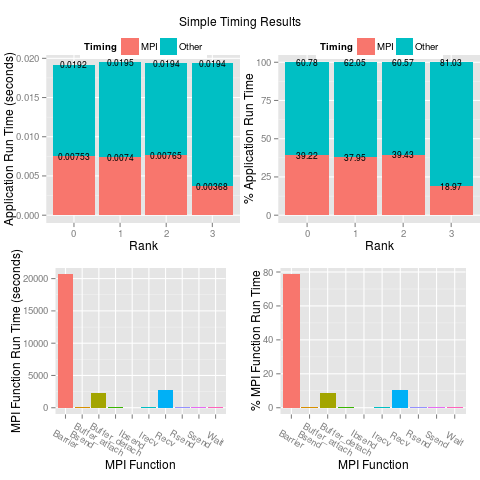
\includegraphics[width=\textwidth]{include/pics/mpip/01_timing}
        \end{subfigure}%
        \hspace{.2cm}
        \begin{subfigure}[b]{0.485\textwidth}
            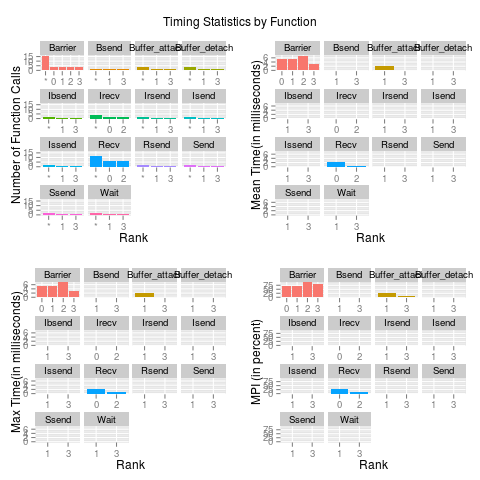
\includegraphics[width=\textwidth]{include/pics/mpip/02_stats}
        \end{subfigure}\\
        \begin{subfigure}[b]{0.485\textwidth}
            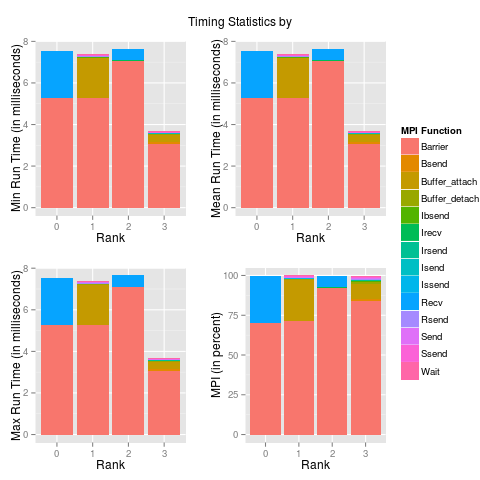
\includegraphics[width=\textwidth]{include/pics/mpip/03_other}
        \end{subfigure}%
        \hspace{.2cm}
        \begin{subfigure}[b]{0.485\textwidth}
            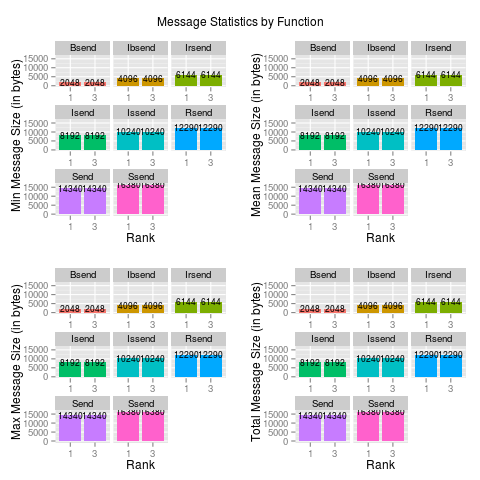
\includegraphics[width=\textwidth]{include/pics/mpip/04_message}
        \end{subfigure}\\
        \begin{subfigure}[b]{0.485\textwidth}
            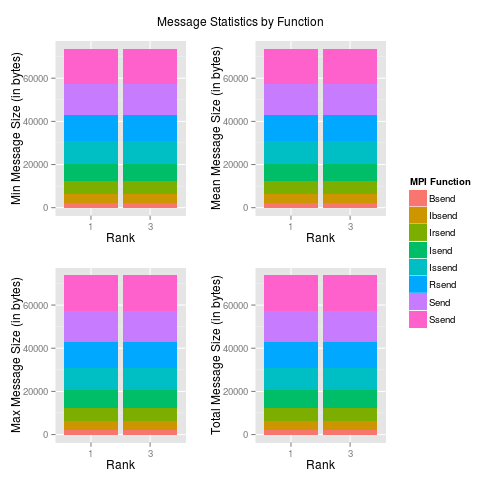
\includegraphics[width=\textwidth]{include/pics/mpip/05_message2}
        \end{subfigure}%
        \caption{mpiP Plots}
        \label{fig:mpip}
\end{figure}


As with fpmpi, both \code{plot()} and \code{autoplot()} methods are available.  For mpiP, there are several different sets of plots available.

Figure~\ref{fig:mpip} shows the 5 different sets of plots which can be produced via the following script.
\begin{lstlisting}[language=rr]
> library(pbdPROF)
> x <- mpip_example
> plot(x, plot.type = "timing", bar.label = T)
> plot(x, plot.type = "stats1", bar.label = T)
> plot(x, plot.type = "stats2", bar.label = T)
> plot(x, plot.type = "messages1", bar.label = T)
> plot(x, plot.type = "messages2", bar.label = T)
\end{lstlisting}
